\chapter{Model-based Reinforcement Learning}
\label{chap4}
\textit{This chapter reviews the details about the implementation of Model-based \ac{RL} for optimal gait control of soft quadruped robots by data-driven methods.}

\section{Neural Networks Design}
The inputs represent features of the input data, each associated with a weight indicating its significance. The transfer function aggregates the weighted inputs, yielding a weighted sum or activation potential. The activation function introduces non-linearity and determines the neuron's output to the network. 

Similar to neural network, an \ac{ANN} consists of interconnected layers of artificial neurons, including the input layer, hidden layers, and output layer, which builds up the world of artificial intelligence. The input layer receives raw data and transfers it to subsequent layers. Hidden layers perform intermediate computations, using activation functions to extract complex features. The output layer produces the final network output based on the assigned task, such as classification or regression. 

Describe the degree project. What did you actually do? This is the practical description of how the method was applied. 
\subsection{Neural Network Architecture}
A fully connected layer refers to a neural network in which each neuron applies a linear transformation to the input vector through a weights matrix. As a result, all possible connections layer-to-layer are present, meaning every input of the input vector influences every output of the output vector. Neural networks are a set of dependent non-linear functions. Each individual function consists of a neuron (or a perceptron). In fully connected layers, the neuron applies a linear transformation to the input vector through a weights matrix. A non-linear transformation is then applied to the product through a non-linear activation function f. $y_{j k}(x)=f\left(\sum_{i=1}^{n_H} w_{j k} x_i+w_{j 0}\right)$
Activation Function: \ac{ReLu} is a commonly used activation function in deep neural networks. It introduces non-linearity into the model, enabling the network to learn complex relationships in the data. \ac{ReLu} applies element-wise activation by setting negative values to zero and leaving positive values unchanged.

Reducing the number of network layers actually weakens the fitting ability of the network

After each fully connected layer, apply the ReLU activation function to introduce non-linearity. This is typically done to enhance the network's representational power and improve its ability to capture complex patterns in the data.
\tikzset{%
  every neuron/.style={
    circle,
    draw,
    minimum size=0.5cm
  },
  neuron missing/.style={
    draw=none, 
    scale=3,
    text height=0.333cm,
    execute at begin node=\color{black}$\vdots$
  },
}

\begin{figure}[ht]
\centering
    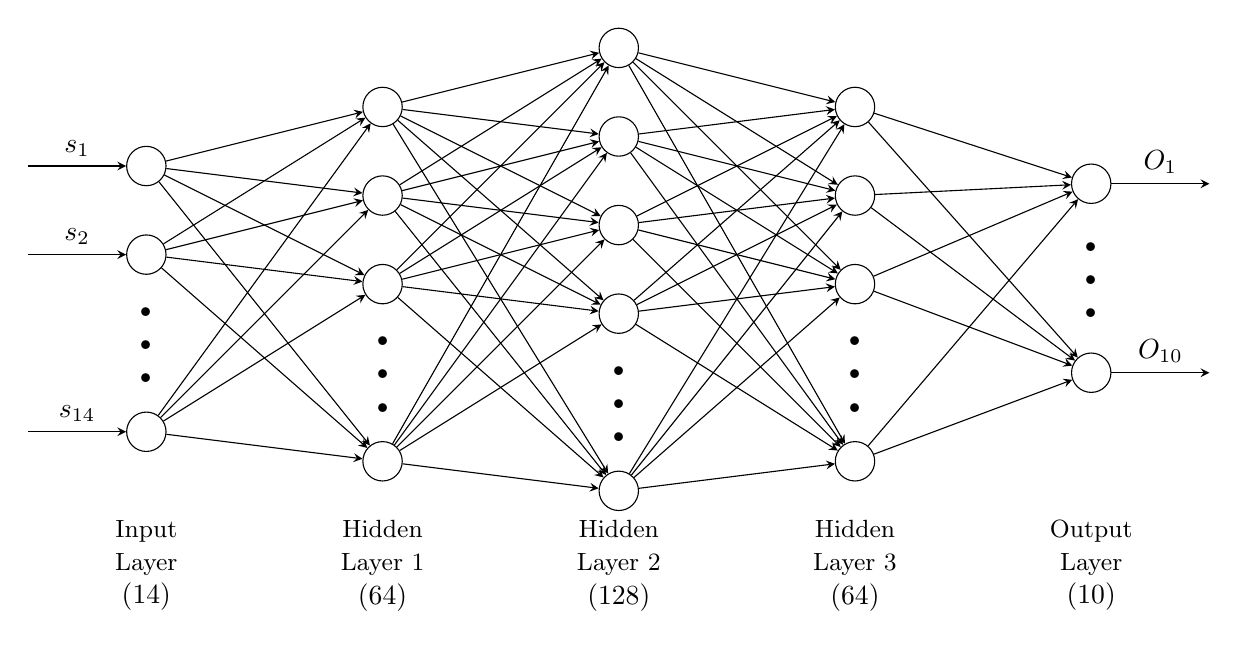
\begin{tikzpicture}[x=1.5cm, y=1.5cm, >=stealth, auto]
    
        \foreach \m/\l [count=\y] in {1,2,missing,3}
          \node [every neuron/.try, neuron \m/.try] (input-\m) at (0,2-\y*.75) {};
        \foreach \m [count=\y] in {1,2,3,missing,4}
          \node [every neuron/.try, neuron \m/.try ] (hidden1-\m) at (2,2.5-\y*0.75) {};
        \foreach \m [count=\y] in {1,2,3,4,missing,5}
          \node [every neuron/.try, neuron \m/.try ] (hidden2-\m) at (4,3-\y*0.75) {};
        \foreach \m [count=\y] in {1,2,3,missing,4}
          \node [every neuron/.try, neuron \m/.try ] (hidden3-\m) at (6,2.5-\y*.75) {};
        \foreach \m [count=\y] in {1,missing,2}
          \node [every neuron/.try, neuron \m/.try ] (output-\m) at (8,1.9-\y*.8) {};
        \foreach \l [count=\i] in {1,2,14}
          \draw [<-] (input-\i) -- ++(-1,0)
            node [above, midway] {$s_{\l}$};
        \foreach \l [count=\i] in {1,10}
          \draw [->] (output-\i) -- ++(1,0)
            node [above, midway] {$O_{\l}$};
        \foreach \i in {1,...,3}
          \foreach \j in {1,...,4}
            \draw [->] (input-\i) -- (hidden1-\j);
        \foreach \i in {1,...,4}
          \foreach \j in {1,...,5}
            \draw [->] (hidden1-\i) -- (hidden2-\j);
        \foreach \i in {1,...,5}
          \foreach \j in {1,...,4}
            \draw [->] (hidden2-\i) -- (hidden3-\j);
        \foreach \i in {1,...,4}
          \foreach \j in {1,...,2}
            \draw [->] (hidden3-\i) -- (output-\j);
        \foreach \l [count=\x from 0] in {\small Input \\\small Layer\\(14) ,\small Hidden \\\small Layer 1\\(64), \small Hidden \\\small Layer 2\\(128), \small Hidden \\\small Layer 3\\(64), \small Output \\\small Layer\\(10)}
          \node [align=center, below, yshift=-5.5cm] at (\x*2,2) {\l};
    \end{tikzpicture}
    \caption{Neural network structure of surrogate model}
    \label{fig:NN}
\end{figure}
        % \foreach \l [count=\i] in {1,2,3,64}
        %   \node [above] at (hidden1-\i.north) {$H_{1,\l}$};
        % \foreach \l [count=\i] in {1,2,3,4,128}
        %   \node [above] at (hidden2-\i.north) {$H_{2,\l}$};
        % \foreach \l [count=\i] in {1,2,3,64}
        %   \node [above] at (hidden3-\i.north) {$H_{3,\l}$};

\subsubsection{loss functions}
Loss functions measure the discrepancy between the predicted outputs of the model and the true labels. The choice of loss function depends on the nature of the task. For multi-class classification problems like yours, common choices include cross-entropy loss and categorical hinge loss. These loss functions encourage the model to output probabilities that align with the true class labels and penalize incorrect predictions.

\subsubsection{Optimization and Validation}
Optimization algorithms are used to update the model's parameters during the training process. Popular optimization algorithms include \ac{SGD}, \ac{Adam}, and \ac{RMSProp}. These algorithms adjust the weights of the model based on the gradients of the loss function with respect to the parameters. They help to guide the model towards finding optimal parameter values that minimize the loss function.

Validation techniques are used to assess the model's performance on unseen data and prevent overfitting. One common approach is to split the available data into training and validation sets. The training set is used to update the model's parameters, while the validation set is used to evaluate the model's performance on data it hasn't seen before. This helps to gauge the generalization ability of the model. Other techniques like k-fold cross-validation and stratified sampling can also be used to ensure robust evaluation.

\subsubsection{Hyperparameters}
Hyperparameters are parameters that are not learned during the training process but are set before training begins. Examples include learning rate, batch size, regularization strength, and the number of hidden layers. Hyperparameter tuning involves systematically varying these parameters and evaluating the model's performance on the validation set. Techniques such as grid search, random search, and Bayesian optimization can be employed to find the optimal values for hyperparameters that yield the best model performance.
Here are some pros and cons of three commonly used optimization algorithms:

\ac{SGD}:
Pros:
It is a simple and computationally efficient optimization algorithm.
It works well for large datasets and can handle noisy or sparse gradients.
It can be used for both shallow and deep neural networks.
Cons:

It may get stuck in local minima and can be slow to converge.
It requires careful tuning of the learning rate.
Adaptive moment estimation (Adam):
Pros:
It is a fast and computationally efficient optimization algorithm.
It uses adaptive learning rates for each parameter and can handle sparse gradients.
It can converge quickly and has been shown to work well for a wide range of deep learning problems.
Cons:

It can converge to sub optimal solutions in some cases.
It may require more memory compared to \ac{SGD}.
Root mean square propagation (RMSprop):
Pros:
It adapts the learning rate based on the average of the recent squared gradients and can handle sparse gradients.
It can converge quickly and has been shown to work well for deep neural networks.
Cons:

It may get stuck in local minima in some cases.
It may require careful tuning of the learning rate and other hyperparameters.
It's important to note that these are just some general pros and cons of each optimization algorithm, and the choice ultimately depends on the specific problem and the network architecture. In practice, it's common to try multiple optimization algorithms and choose the one that works best for the specific problem.

The learning rate defines the size of the corrective steps that the model takes to adjust for errors in each observation. A high learning rate shortens the training time, but with lower ultimate accuracy, while a lower learning rate takes longer, but with the potential for greater accuracy. Optimizations such as Quickprop are primarily aimed at speeding up error minimization, while other improvements mainly try to increase reliability. In order to avoid oscillation inside the network such as alternating connection weights, and to improve the rate of convergence, refinements use an adaptive learning rate that increases or decreases as appropriate. The concept of momentum allows the balance between the gradient and the previous change to be weighted such that the weight adjustment depends to some degree on the previous change. A momentum close to 0 emphasizes the gradient, while a value close to 1 emphasizes the last change.

While it is possible to define a cost function ad hoc, frequently the choice is determined by the function's desirable properties (such as convexity) or because it arises from the model (e.g. in a probabilistic model the model's posterior probability can be used as an inverse cost).

Backpropagation is a method used to adjust the connection weights to compensate for each error found during learning. The error amount is effectively divided among the connections. Technically, backprop calculates the gradient (the derivative) of the cost function associated with a given state with respect to the weights. The weight updates can be done via stochastic gradient descent or other methods, such as Extreme Learning Machines, "No-prop" networks, training without backtracking, "weightless" networks, and non-connectionist neural networks

Stochastic gradient descent (SGD) is an iterative optimization algorithm commonly used in machine learning to train neural networks. It is a variant of gradient descent that updates the model parameters (weights and biases) on a per-sample basis, rather than accumulating the gradients over the entire training set.

In SGD, the training data is typically divided into small batches (mini-batches), and the model parameters are updated after processing each batch. The algorithm computes the gradient of the loss function with respect to the parameters using the current mini-batch, and then updates the parameters by taking a step in the direction of the negative gradient.

The advantage of SGD is that it can converge faster than batch gradient descent, especially when the training set is large. It also has lower memory requirements, since only a small batch of training data needs to be loaded into memory at a time.

However, the updates in SGD can be noisy due to the small batch size, which can lead to instability and oscillations in the training process. To mitigate this issue, several variants of SGD have been proposed, such as momentum-based methods, adaptive learning rate methods (e.g., Adam, Adagrad), and variants that combine multiple mini-batches (e.g., mini-batch gradient descent).
Here are some general pros and cons of some commonly used optimization algorithms in deep learning:

Stochastic Gradient Descent (SGD):
Pros:
Simple and easy to implement.
Fast convergence on simple problems.
Cons:

Can converge slowly on problems with more complex and non-convex loss surfaces.
Can get stuck in local minima.
Adaptive Moment Estimation (Adam):
Pros:
Efficient and performs well on a wide range of problems.
Adapts to the shape of the loss surface and can handle noisy gradients.
Cons:

Can converge to suboptimal solutions.
May require some tuning of the learning rate and momentum hyperparameters.
Nesterov Accelerated Gradient (NAG):
Pros:
Can converge faster than traditional SGD.
Resilient to high condition number and high curvature problems.
Cons:

Slightly more complex than traditional SGD.
Can be sensitive to the choice of momentum hyperparameter.
Root Mean Square Propagation (RMSprop):
Pros:
Efficient and performs well on a wide range of problems.
Adapts to the shape of the loss surface and can handle noisy gradients.
Cons:

Can converge to suboptimal solutions.
May require some tuning of the learning rate and momentum hyperparameters.
Adaptive Gradient Algorithm (AdaGrad):
Pros:
Efficient and performs well on sparse datasets.
Adapts to the shape of the loss surface and can handle noisy gradients.
Cons:

May converge too quickly on some problems and not converge at all on others.
May require some tuning of the learning rate hyperparameter.
Limited-memory Broyden-Fletcher-Goldfarb-Shanno (L-BFGS):
Pros:
Converges quickly and efficiently on smooth, non-convex optimization problems.
Doesn't require the learning rate hyperparameter.
Cons:

Can be computationally expensive and memory-intensive for large datasets.
Can get stuck in local minima.
\subsection{Potential Reality Gap}
blabla

\section{Model-based RL Algorithm}

\section{Validation}

\section{Control architecture Design}
\subsection{Task Planning and Execution}

